\titledquestion{Dijkstra}[8]
Given the following weighted graph, run Dijkstra's algorithm by considering $A$ as the source vertex. Write down the vertex you select and update the distance \texttt{dis[i]} of all vertices in each iteration.

\begin{figure}[htbp]
    \centering
    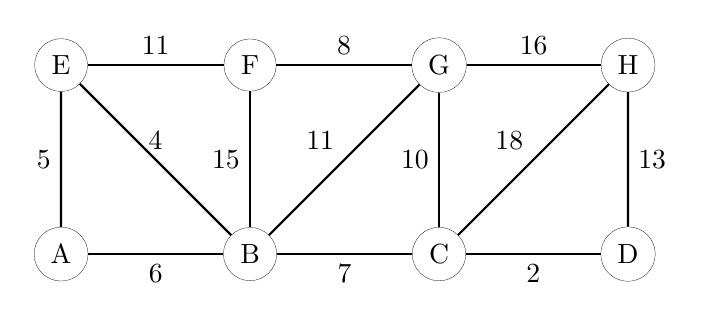
\begin{tikzpicture}
    [thick,scale=0.8, every node/.style={scale=1}]
    %		\node[circle] (n0){A};
    \node[circle, draw, line width=0.1pt] (a) at (-4.5,0){A};
    \node[circle, draw, line width=0.1pt] (b) at (-1.5,0){B};
    \node[circle, draw, line width=0.1pt] (c) at (1.5,0){C};
    \node[circle, draw, line width=0.1pt] (d) at (4.5,0){D};
    \node[circle, draw, line width=0.1pt] (e) at (-4.5,3){E};
    \node[circle, draw, line width=0.1pt] (f) at (-1.5,3){F};
    \node[circle, draw, line width=0.1pt] (g) at (1.5,3){G};
    \node[circle, draw, line width=0.1pt] (h) at (4.5,3){H};
    \draw[-] (a) to node[below]{6} (b);
    \draw[-] (a) to node[left]{5} (e);
    \draw[-] (b) to node[below]{7} (c);
    \draw[-] (b) to node[above]{4} (e);
    \draw[-] (b) to node[left]{15} (f);
    \draw[-] (b) to node[above left]{11} (g);
    \draw[-] (c) to node[below]{2} (d);
    \draw[-] (c) to node[left]{10} (g);
    \draw[-] (c) to node[above left]{18} (h);
    \draw[-] (d) to node[right]{13} (h);
    \draw[-] (e) to node[above]{11} (f);
    \draw[-] (f) to node[above]{8} (g);
    \draw[-] (g) to node[above]{16} (h);
    \end{tikzpicture}
\end{figure}
\vspace{0.5cm}


Fill in the table below.
\begin{table}[htbp]
    \begin{center}  
        \begin{tabular}{|l|c|c|c|c|c|c|c|c|c| p{3cm}|}  
            \hline  
            & vertex & \texttt{dis[A]} & \texttt{dis[B]} & \texttt{dis[C]} & \texttt{dis[D]} & \texttt{dis[E]} & \texttt{dis[F]} & \texttt{dis[G]} & \texttt{dis[H]}\\ \hline  
            initial 	& / & 0 &$\infty$&$\infty$&$\infty$&$\infty$&$\infty$&$\infty$&$\infty$\\ \hline
            iteration 1 & A  & 0  & 6  & $\infty$  & $\infty$  & 5  & $\infty$  &  $\infty$ & $\infty$ \\ \hline    
            iteration 2 & E  & 0  & 6  & $\infty$  & $\infty$  & 5  & 16  & $\infty$  & $\infty$ \\ \hline    
            iteration 3 & B  & 0  & 6  & 13  & $\infty$  & 5  & 16  &  17 & $\infty$ \\ \hline    
            iteration 4 & C  & 0  & 6  & 13  & 15  & 5  & 16  & 17 & 31 \\ \hline    
            iteration 5 & D  & 0  & 6  & 13  & 15  & 5  & 16  & 17  & 28 \\ \hline   
            iteration 6 & F  & 0  & 6  & 13  & 15  & 5  & 16  & 17  & 28 \\ \hline    
            iteration 7 & G  & 0  & 6  & 13  & 15  & 5  & 16  & 17  & 28 \\ \hline   
            iteration 8 & H  & 0  & 6  & 13  & 15  & 5  & 16  & 17  & 28 \\  
            \hline  
        \end{tabular}  
    \end{center}  
\end{table}
